\appendix
\chapter{Null space inverse kinematics}
\label{apx:null-space}
As discussed in \refsec{sec:trajectories}, inverse kinematics will be an underdetermined system if the number of controllable joints exceeds the degrees of freedom of the desired end effector pose. This has the effect of having infinitely many, all equally valid robot poses which achieve the desired end effector position. However, this is only in theory. Consider \reffig{fig:ik-invalid}. Here we can see that the solution requires two of the arm links to intersect. While this is fine in theory and does constitute a solution to the IK system, in the real world the links of the robot arm are not infinitely thin line segments, they are physical parts with thickness. If this robot was in the real world this would require parts of the robot to pass through each other. This is obviously impossible in a real situation.

\begin{figure}[h]
    \centering
    \begin{subfigure}[b]{0.45\textwidth}
        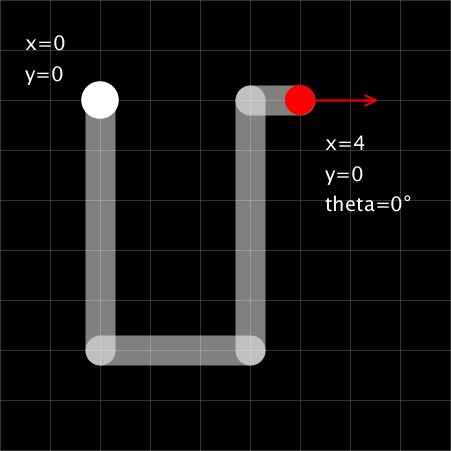
\includegraphics[width=\textwidth]{figures/ik-valid.png}
        \caption{A valid IK solution}
        \label{fig:ik-valid}
    \end{subfigure}
    \hfill
    \begin{subfigure}[b]{0.45\textwidth}
        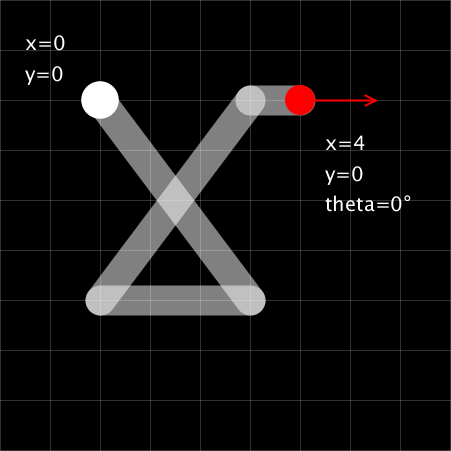
\includegraphics[width=\textwidth]{figures/ik-invalid.png}
        \caption{An invalid IK solution}
        \label{fig:ik-invalid}
    \end{subfigure}
    \caption{Not all IK solutions may be valid}
    \label{fig:ik-null-space}
\end{figure}

Fortunately for us, we saw that by having additional degrees of freedom, we can generate infinitely many solutions to the IK system. This means we could prune these invalid solutions by adding additional constraints. While it is possible this could make all solutions invalid, this is both unlikely and necessary. These invalid solutions remain because the current IK system does not perfectly capture our real world restrictions. If all solutions are removed by our additional constraints, then this simply means the desired end effector pose was not possible in a real world system.\\

There are two main ...